%%%%%%%%%%%%%%%%%%%%%%%%%%%%%%%%%%%%%%%%
% 
% DND tex file generated from alg_spec.dndspec
%
%%%%%%%%%%%%%%%%%%%%%%%%%%%%%%%%%%%%%%%%

%
% algorithm specification
%
% EXTRA_HEADER_TEX: \setlength{\textwidth}{4.0in}
% ALL_LABELS:   {s_1}, {\sigma_1}, {\sigma_3}, {\alpha_1}, {\sigma_2}, {\alpha_2}


\documentclass{article}
\usepackage[margin=0.6in, paperwidth=11in, paperheight=4.6in]{geometry}
\usepackage{amsmath}

\usepackage{amsmath}
\usepackage{amssymb}
\usepackage{tikz}
\usetikzlibrary{shapes.geometric, arrows.meta, positioning, fit, backgrounds, calc}
%%% TikZ styles %%%
\tikzset{
  specbox/.style={
    draw, rectangle, minimum width=2.4cm, minimum height=0.9cm,
    text centered, font=\small, inner sep=4pt, line width=0.6pt
  },
  procbox/.style={
    draw, rectangle, minimum width=4.2cm,
    text centered, font=\small, inner sep=8pt, line width=0.6pt,
    align=center
  },
  sectionlabel/.style={
    font=\small\bfseries, text centered
  },
  arrow/.style={
    ->, >=Stealth, line width=0.6pt
  },
  statearrow/.style={
    ->, >=Stealth, line width=0.6pt, dashed
  },
}


\input{latex2dnd}

\def\lbL{\lb\rule{0pt}{2.4ex}}
\def\lpL{\left(\rule{0pt}{2.4ex}}
\def\lb{\left[}         \def\rb{\right]}
\def\lp{\left(}         \def\rp{\right)}
\def\rar{\rightarrow}
\def\del{\nabla}
\def\w{\omegaup}
\def\ket#1{\left\vert #1 \right\rangle}
\def\bra#1{\left\langle #1 \right\vert}
\def\M#1#2{M_{#1}( #2) }
\def\R#1#2{R_{#1}( #2 ) }
\def\adag{a^\dagger}
\def\bdag{b^\dagger}
\def\Bdag{B^\dagger}

\def\bea{\begin{eqnarray}}
\def\eea{\end{eqnarray}}
\def\ben{\begin{eqnarray*}}
\def\een{\end{eqnarray*}}

\def\non{\nonumber}

\def\>{\rangle}
\def\<{\langle}
\def\l{\left}
\def\r{\right}

%%%%%%%%%%%%%%%%%%%%%%%%%%%%%%%%%%%%%%%%%%%%%%%%%%%%%%%%%%%%%%%%%%%%%%%%%%%%%

\newsavebox{\DBXaa}
\newsavebox{\DBXab}
\newsavebox{\DBXac}
\newsavebox{\DBXad}

%%%%%%%%%%%%%%%%%%%%%%%%%%%%%%%%%%%%%%%%%%%%%%%%%%%%%%%%%%%%%%%%%%%%%%%%%%%%%

\begin{document}

%%%%%%%%%%%%%%%%%%%%%%%%%%%%%%%%%%%%%%%%
% OPTIONS
%%%%%%%%%%%%%%%%%%%%%%%%%%%%%%%%%%%%%%%%

% \DDoptions{ALLOW_EMPTY}
% \DDoptions{DD_HIDE_FORMULA_INPUT}
\DDoptions{HIDE_FORMULA_INPUT}

% Resolution: 300

%%%%%%%%%%%%%%%%%%%%%%%%%%%%%%%%%%%%%%%%
% define drag-drop labels
%%%%%%%%%%%%%%%%%%%%%%%%%%%%%%%%%%%%%%%%

\DDlabel[un]{un}{${u^n}$}
\DDlabel[a]{a}{${a}$}
\DDlabel[unplus1]{unplusone}{${u^{n+1}}$}

%%%%%%%%%%%%%%%%%%%%%%%%%%%%%%%%%%%%%%%%
% shorthand macro to make boxes the same size
%
% edit these if boxes too small
%%%%%%%%%%%%%%%%%%%%%%%%%%%%%%%%%%%%%%%%
\newcommand\DDB[2]{\DDbox{#1}{8ex}{4ex}{#2}}
\newcommand\DDBB[2]{\DDbox{#1}{12ex}{6ex}{#2}}
\newcommand\DDBBB[2]{\DDbox{#1}{12ex}{6ex}{#2}}
\newcommand\DDBBBB[2]{\DDbox{#1}{14ex}{6ex}{#2}}

\savebox{\DBXaa}{\DDB{1}{un}}
\savebox{\DBXab}{\DDB{2}{a}}
\savebox{\DBXac}{\DDB{3}{unplusone}}
\savebox{\DBXad}{\DDB{4}{unplusone}}

%%%%%%%%%%%%%%%%%%%%%%%%%%%%%%%%%%%%%%%%
% original expression, for reference
%%%%%%%%%%%%%%%%%%%%%%%%%%%%%%%%%%%%%%%%

%\begin{center}
%\begin{tikzpicture}[node distance=0.55cm and 1.0cm]
%
%  %%% PROCEDURE box (center) %%%
%  \node[procbox, align=left] (proc) {%
%    \textbf{for} $i = 1, \ldots, N-2$:\\[2pt]
%    $\quad\mathrm{tmp}[i] = u^n_i $\\[3pt]
%    $~~~~~~~~~~ + a\bigl(u^n_{i-1} - 2u^n_i + u^n_{i+1}\bigr)$\\[4pt]
%    $ {u^{n+1}} \leftarrow \mathrm{tmp}$
%  };
%
%  %%% INPUT boxes (left of procedure) %%%
%  \node[specbox, left=1.4cm of proc, yshift=0.9cm] (in1)
%    {current array $ {u^n} $};
%
%  \node[specbox, below=of in1] (in2)
%    {parameter $ {a} $};
%
%  \node[specbox, below=of in2] (in3)
%    {boundary values};
%
%  %%% OUTPUT box (right of procedure) %%%
%  \node[specbox, right=1.4cm of proc] (out)
%    {updated array $ {u^{n+1}} %};
%
%  %%% Section labels %%%
%  \node[sectionlabel, above=0.5cm of in1, xshift=0.0cm] (lbl_in)
%    {INPUTS};
%
%  \node[sectionlabel, above=0.5cm of proc] (lbl_proc)
%    {PROCEDURE};
%
%  \node[sectionlabel, above=0.5cm of out] (lbl_out)
%    {OUTPUT};
%
%  %%% Arrows: inputs → procedure %%%
%  \draw[arrow] (in1.east) -- ++(0.5,0) |- (proc.west);
%  \draw[arrow] (in2.east) -- ++(0.5,0) |- (proc.west);
%  \draw[arrow] (in3.east) -- ++(0.5,0) |- (proc.west);
%
%  %%% Arrow: procedure → output %%%
%  \draw[arrow] (proc.east) -- (out.west);
%
%  %%% Outer frame %%%
%  \begin{scope}[on background layer]
%    \node[draw, dashed, inner sep=10pt, line width=0.5pt,
%          fit=(lbl_in)(lbl_proc)(lbl_out)(in3)(out)(proc)](outerbox){};
%  \end{scope}
%
%  %%% Algorithm name above the outer frame %%%
%  \node[font=\normalsize\bfseries, above=6pt of outerbox.north]
%    {ONE STEP: 1-D DIFFUSION ALGORITHM};
%
%  %%% STATE box (below outer frame) %%%
%%  \node[specbox, minimum width=2.8cm, below=0.65cm of outerbox.south,
%%        xshift=-1.4cm] (state)
%%    {current array $u^n$};
%
%%  \node[sectionlabel, left=0.25cm of state] {STATE:};
%
%  %%% State arrow: output → down → left → state %%%
%%  \coordinate (corner) at ($(out.south) + (0,-0.55)$);
%%  \draw[statearrow] (out.south) -- (corner)
%%    -- ($(state.east |- corner)$) -- (state.east);
%
%\end{tikzpicture}
%\end{center}
%
%

%%%%%%%%%%%%%%%%%%%%%%%%%%%%%%%%%%%%%%%%
% dnd expression with boxes
%%%%%%%%%%%%%%%%%%%%%%%%%%%%%%%%%%%%%%%%

%\begin{center}
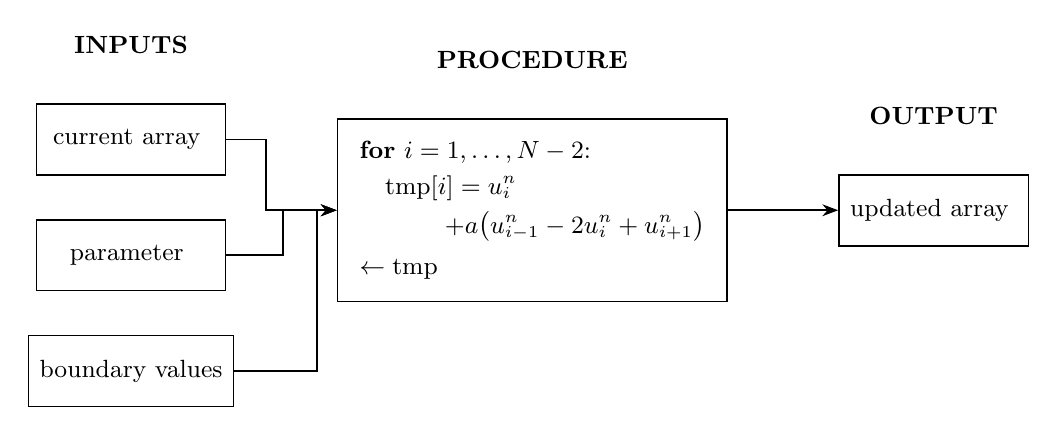
\begin{tikzpicture}[node distance=0.55cm and 1.0cm]

  %%% PROCEDURE box (center) %%%
  \node[procbox, align=left] (proc) {%
    \textbf{for} $i = 1, \ldots, N-2$:\\[2pt]
    $\quad\mathrm{tmp}[i] = u^n_i $\\[3pt]
    $~~~~~~~~~~ + a\bigl(u^n_{i-1} - 2u^n_i + u^n_{i+1}\bigr)$\\[4pt]
    $ \usebox{\DBXac} \leftarrow \mathrm{tmp}$
  };

  %%% INPUT boxes (left of procedure) %%%
  \node[specbox, left=1.4cm of proc, yshift=0.9cm] (in1)
    {current array $ \usebox{\DBXaa} $};

  \node[specbox, below=of in1] (in2)
    {parameter $ \usebox{\DBXab} $};

  \node[specbox, below=of in2] (in3)
    {boundary values};

  %%% OUTPUT box (right of procedure) %%%
  \node[specbox, right=1.4cm of proc] (out)
    {updated array $ \usebox{\DBXad} $};

  %%% Section labels %%%
  \node[sectionlabel, above=0.5cm of in1, xshift=0.0cm] (lbl_in)
    {INPUTS};

  \node[sectionlabel, above=0.5cm of proc] (lbl_proc)
    {PROCEDURE};

  \node[sectionlabel, above=0.5cm of out] (lbl_out)
    {OUTPUT};

  %%% Arrows: inputs → procedure %%%
  \draw[arrow] (in1.east) -- ++(0.5,0) |- (proc.west);
  \draw[arrow] (in2.east) -- ++(0.720,0) |- (proc.west);
  \draw[arrow] (in3.east) -- ++(1.05,0) |- (proc.west);

  %%% Arrow: procedure → output %%%
  \draw[arrow] (proc.east) -- (out.west);

  %%% Outer frame %%%
%  \begin{scope}[on background layer]
%    \node[draw, dashed, inner sep=10pt, line width=0.5pt,
%          fit=(lbl_in)(lbl_proc)(lbl_out)(in3)(out)(proc)](outerbox){};
%  \end{scope}

  %%% Algorithm name above the outer frame %%%
%  \node[font=\normalsize\bfseries, above=6pt of outerbox.north]
%    {ONE STEP: 1-D DIFFUSION ALGORITHM};

  %%% STATE box (below outer frame) %%%
%  \node[specbox, minimum width=2.8cm, below=0.65cm of outerbox.south,
%        xshift=-1.4cm] (state)
%    {current array $u^n$};

%  \node[sectionlabel, left=0.25cm of state] {STATE:};

  %%% State arrow: output → down → left → state %%%
%  \coordinate (corner) at ($(out.south) + (0,-0.55)$);
%  \draw[statearrow] (out.south) -- (corner)
%    -- ($(state.east |- corner)$) -- (state.east);

\end{tikzpicture}
%\end{center}


%%%%%%%%%%%%%%%%%%%%%%%%%%%%%%%%%%%%%%%%
% dnd check formula
%%%%%%%%%%%%%%%%%%%%%%%%%%%%%%%%%%%%%%%%


%%%%%%%%%%%%%%%%%%%%%%%%%%%%%%%%%%%%%%%%
% dnd formula tests
%%%%%%%%%%%%%%%%%%%%%%%%%%%%%%%%%%%%%%%%


%%%%%%%%%%%%%%%%%%%%%%%%%%%%%%%%%%%%%%%%
% dnd feedback
%%%%%%%%%%%%%%%%%%%%%%%%%%%%%%%%%%%%%%%%


%%%%%%%%%%%%%%%%%%%%%%%%%%%%%%%%%%%%%%%%
% output labels, with fixed box heights
%%%%%%%%%%%%%%%%%%%%%%%%%%%%%%%%%%%%%%%%
\writeDDlabels[4.3ex]

\end{document}
%%%%%%%%%%%%%%%%%%%%%%%%%%%%%%%%%%%%%%%%%%%%%%%%%%%%%%%%%%%%%%%%%%%%%%%%%%%%%

